%% \documentclass[authoryear,preprint,review,12pt]{elsarticle}
\documentclass[preprint,letterpaper]{elsarticle}


%-------- packages --------

\usepackage{amsmath}
\usepackage{amssymb}
\usepackage{hyperref}
\usepackage{lineno}                 % line numbers
\usepackage[version=4]{mhchem}      % chem formatting
\usepackage{siunitx}                % units formatting
\usepackage{rotating}
%\usepackage{longtable}
%\usepackage{float}
%\usepackage{caption}
\usepackage{tabularx}
\usepackage{fontawesome}
\usepackage{enumitem}
\usepackage{graphicx}
\usepackage{textcomp}
\usepackage{booktabs}               % table rules
\setlist{itemsep=0pt}

%-------- package setup --------

\sisetup{exponent-mode = scientific}

%-------- more units --------

\DeclareSIUnit\atm{atm}
\DeclareSIUnit\atmosphere{atm}
\DeclareSIUnit\amu{amu}
\DeclareSIUnit\atomicmassunit{amu}

\newcommand{\prtl}[2]{\frac{\partial #1}{\partial #2}}

%-------- front matter --------

\journal{SoftwareX}

\begin{document}

\begin{frontmatter}

%% Title, authors and addresses

%% use the tnoteref command within \title for footnotes;
%% use the tnotetext command for theassociated footnote;
%% use the fnref command within \author or \address for footnotes;
%% use the fntext command for theassociated footnote;
%% use the corref command within \author for corresponding author footnotes;
%% use the cortext command for theassociated footnote;
%% use the ead command for the email address,
%% and the form \ead[url] for the home page:
%% \title{Title\tnoteref{label1}}
%% \tnotetext[label1]{}
%% \author{Name\corref{cor1}\fnref{label2}}
%% \ead{email address}
%% \ead[url]{home page}
%% \fntext[label2]{}
%% \cortext[cor1]{}
%% \address{Address\fnref{label3}}
%% \fntext[label3]{}

\title{SootLib: a soot model library for combustion and reacting flow simulation}

%% use optional labels to link authors explicitly to addresses:
%% \author[label1,label2]{}
%% \address[label1]{}
%% \address[label2]{}

%\renewcommand{\thefootnote}{\fnsymbol{footnote}}
\author{Victoria B. Stephens}
\author{Joshua Bedwell}
\author{Alex J. Josephson}
\author{Keturah Oldham}
\author{David O. Lignell\corref{cor1}}

\cortext[cor1]{Corresponding author \ead{davidlignell@byu.edu}}

\address{Chemical Engineering Department, Brigham Young University, Provo, UT 84602, USA}

%%%%%%%%%%%%%%%%%%%%%%%%%%%%%%%%%%%%%%%%%%%%%%%%%%%%%%%%%%%%%%%%%%%%%%%%%%%%%%%

\begin{abstract}
%
Soot formation in combustion is an important process that affects radiative heat transfer, flame temperatures, and emissions with health and environmental impacts. Soot formation involves complex chemistry for nucleation, growth, oxidation, and coagulation processes. The soot particles vary widely in size and accurate modeling requires representation of the particle size distribution (PSD). Modeling soot is not trivial, and is only one of several physical processes active in combustion systems. This paper presents a software package called SootLib, which is an open-source library for modeling soot formation and other aerosol systems. SootLib is written in C++, is documented with Doxygen, and is available on GitHub. The library includes several models for soot chemistry and coagulation, and it represents the PSD using either a sectional model or the method of moments (MOM). Four closure approaches for the MOM are implemented allowing up to eight moments: monodispersed, an assumed-shape lognormal distribution, the quadrature method of moments, and the method of moments with interpolative closure. SootLib provides an interface for inclusion in other combustion packages including CFD or reacting flow solvers. The range of of models allows comparisons and sensitivity studies, and the modularity facilitates extension to other soot models.
%
\end{abstract}

\begin{keyword}
soot \sep combustion \sep simulation \sep aerosol
\end{keyword}

\end{frontmatter}

\linenumbers

%%%%%%%%%%%%%%%%%%%%%%%%%%%%%%%%%%%%%%%%%%%%%%%%%%%%%%%%%%%%%%%%%%%%%%%%%%%%%%%

\section{Introduction}
\label{s:intro}

Soot formation is a fundamental aspect of non-premixed combustion that is important in many engineering applications, including wildland fires. Soot is responsible for a flame's luminosity, generates a large portion of a flame's radiative heat transfer to its surroundings, and contributes to many of the health, safety, and environmental hazards associated with air pollution from combustion systems~\cite{EPA_2009,EPA_2004}. In order to address soot's negative effects and optimize practical combustion processes, scientists and engineers seek a better understanding of soot's fundamental structure and behavior in combustion environments, often through modeling and simulation.
Combustion processes span many orders of magnitude in both their length and time scales, and simulating soot in flames further expands the range of scales that must be considered, adding additional complexity and computational cost.

Direct simulation approaches can produce accurate simulation data by resolving the full range of length and time scales, but the computational cost can be prohibitively high, particularly for simulating practical combustion processes of interest to engineers~\cite{Pope_2000}.
Computational models that quantify soot production in simulations can help us study its fundamental behavior and distinguish between various reaction mechanisms and transport models while also reducing the potentially high computational cost. Such models represent an important step forward in the study of combustion systems ~\cite{Frenklach_2002b}.

This paper presents SootLib, an easy-to-use software package that serves as an access point for soot property and particle dynamics modeling and can be interfaced with various simulation approaches for combustion CFD.
SootLib is a C++ library with a modular design featuring interchangeable model parts, allowing users to quickly and easily compare and contrast models within its library of validated mechanisms for soot chemistry and particle dynamics, all of which are implemented with a consistent interface.
SootLib includes models for soot chemistry as well as representations of the particle size distribution (PSD), including a sectional model and the method of moments (MOM) with four closure schemes that consider up to eight moments.
While focused on soot formation in combustion systems, SootLib can be applied broadly to a range of aerosol systems.
We present below a summary of the soot models, a description of the SootLib software, and illustrative examples.

%%%%%%%%%%%%%%%%%%%%%%%%%%%%%%%%%%%%%%%%%%%%%%%%%%%%%%%%%%%%%%%%%%%%%%%%%%%%%%%

\section{Model Descriptions}
\label{s:models}

In general, soot models can be broken down into two interrelated parts: chemistry and particle dynamics.
Soot chemistry models address the chemical reactions involved in soot behavior, including particle inception, growth, and destruction, while particle dynamics models describe the soot particle size distribution (PSD) and its evolution.
Using a particular set of soot chemistry models generally does not necessitate using a particular PSD model.
SootLib has a modular structure that allows users to specify individual models rather than predetermined model sets, giving users more flexibility and facilitating model comparisons and sensitivity analysis.

%%%%%%%%%%%%%%%%%%%%%%%%%%%%%%%%%%%%%%%%%%%%%%%%%%%%%%%%%%%%%%%%%%%%%%%%%%%%%%%

\subsection{Chemistry}
\label{s:chemistry}

In combustion modeling contexts, soot is usually described as a collection of carbon atoms above a predefined mass threshold.\footnote{In reality, soot also contains lesser amounts of hydrogen and other elements.} Soot particles are typically assumed to be spherical, which facilitates calculation of particle diameter, volume, and surface area.\footnote{This is a reasonable assumption for nascent soot particles, but may not be adequate to describe large soot agglomerates, which tend to exhibit fractal structures~\cite{Jullien_1987,Wang_2011}.}

Soot chemistry is commonly divided into four categories, all of which depend on and influence the soot PSD and the gas state: nucleation from gaseous precursors,\footnote{Soot produced by liquid or solid fuels nucleates by different mechanisms. At this time, SootLib's models only apply to gaseous fuels.} growth and oxidation of soot by reaction with gaseous species, and coagulation of soot particles to form larger particles.
Additional soot processes include growth by condensation of polycyclic aromatic hydrocarbons (PAH), agglomeration into large fractal aggregates, and fragmentation during oxidation processes.
Some models provide all four mechanisms, while others expand on earlier mechanisms or focus on one type.

Global kinetic mechanisms, typically represented by Arrhenius-style rate expressions, do not capture all of the fundamental mechanisms of soot phenomena, but they are relatively simple, easy to implement, and computationally inexpensive, making them popular choices in combustion simulations involving soot.
In other words, global models tend to sacrifice accuracy in favor of high speed and low computational cost.
Physics-based models and mechanisms use multiple elementary reaction steps to represent actual soot behavior rather than relying on the empiricism inherent in global reaction models.
By accounting for fundamental phenomena, physics-based models may result in increased accuracy at the expense of computational speed and efficiency.

SootLib collects a range of models from the literature and implements them with a uniform interface, offering modelers a flexible framework for model development and simulation. Table~\ref{t:chem_models} summarizes the soot chemistry models implemented in SootLib, and the following sections provide general descriptions. Further information is provided in the package documentation.

%
\begin{sidewaystable}
\caption[Summary of soot chemistry models implemented in SootLib]{Summary of soot chemistry models implemented in SootLib. In mechanisms, \ce{C(s)} represents a soot particle, i.e. ``solid'' carbon, and \ce{C(s)^.} indicates a radical site on a soot particle, typically caused by hydrogen abstraction. Variable definitions for rate expressions and rate expressions that involve multiple expressions or otherwise do not fit well in this table can be found in their respective sections as noted.}
    \label{t:chem_models}
    \centering
    \resizebox{\textwidth}{!}{
        \begin{tabular}{l l l l l}
            \toprule
            Chemistry type  & Model                 & Model ID     & Mechanism & Rate expression \\
            \midrule
            Nucleation      & Leung \& Lindstedt~\cite{Leung_1991}  & \texttt{LL}    & \ce{C2H2 -> 2C(s) + H2} & $R_{nuc} = 0.1\times 10^5 e^{-21100/T} \ce{[C2H2]}$\\
            & Lindstedt 2005~\cite{Lindstedt_2005}  & \texttt{LIN}   & \ce{C2H2 -> 2C(s) + H2} & $R_{nuc} = 0.63\times 10^4 e^{-21100/T} \ce{[C2H2]}$\\
            & PAH nucleation~\cite{Blanquart_2009}  & \texttt{PAH}  & \ce{PAH + PAH -> DIMER} & \\
            &  &  & \ce{DIMER + DIMER -> C(s)} & $R_{nuc} = 0.5\beta_{D,D} n_D^2$  \\
            \midrule
            Surface growth  & Leung \& Lindstedt~\cite{Leung_1991}  & \texttt{LL}    & \ce{C2H2 + nC(s) ->} (n+2)\ce{C(s) + H2} & $R_{grw} = \num{0.6e4} e^{-12100/T} f(A_s) \ce{[C2H2]}$\\
            & Lindstedt 1994~\cite{Lindstedt_1994}  & \texttt{LIN}   & \ce{C2H2 + nC(s) ->} (n+2)\ce{C(s) + H2} & $R_{grw} = \num{0.1e-11} e^{-12100/T} \ce{[C2H2]} 2M_0 MW_C$ \\
            & HACA~\cite{Appel_2000,Frenklach_1994} & \texttt{HACA}  & \ce{C(s)-H + H <=> C(s)^. + H2}   & $R_{grw,f}=\num{4.2e13} e^{-13/RT} \ce{[H]}$ \\
            &                                       &                &                                   & $R_{grw,r}=\num{3.9e12} e^{-11/RT} \ce{[H2]}$ \\
            &                                       &                & \ce{C(s)-H + OH <=> C(s)^. + H2O} & $R_{grw,f}=\num{1e10} T^{0.734} e^{-1.43/RT} \ce{[OH]}$ \\
            &                                       &                &                                   & $R_{grw,r}=\num{3.68e8} T^{1.139} e^{-17.1/RT} \ce{[H2O]}$ \\
            &                                       &                & \ce{C(s)^. + H -> C(s)-H}         & $R_{grw}=\num{2.0e13} \ce{[H]}$ \\
            &                                       &                & \ce{C(s)^. + C2H2 -> C(s)-H + H}  & $R_{grw}=\num{8.0e7} T^{1.56} e^{-3.8/RT} \ce{[C2H2]}$\\

            \midrule
            Oxidation       & Leung \& Lindstedt~\cite{Leung_1991}   & \texttt{LL}   &  \ce{C(s) + 1/2O2 -> CO} & $R_{oxi,\ce{O2}} = \num{0.1e5} T^{1/2} e^{-19680/T} \ce{[O2]}$\\
            & HACA~\cite{Appel_2000,Frenklach_1994} & \texttt{HACA}  & \ce{C(s)^. + O2 -> 2CO + products} & $R_{oxi,\ce{O2}}=\num{2.2e12} e^{-7.5/RT} \ce{[O2]}$\\
            &                                       &                & \ce{C(s)-H + OH -> CO + products} & $R_{oxi,\ce{OH}}=0.13\cdot 1290 P_{\ce{OH}} T^{-1/2} $\\
            & Lee~\cite{Lee_1962} +
            Neoh~\cite{Neoh_1980,Neoh_1981}       & \texttt{LEE\textunderscore NEOH} & \ce{C + 1/2O2 -> CO} & $R_{oxi,\ce{O2}} = \num{1.085e4} P_{\ce{O2}} T^{-1/2} e^{-19778.24/T}$\\
            &                                       &                & \ce{C + OH -> CO + H} & $R_{oxi,\ce{OH}}=0.13\cdot 1290 P_{\ce{OH}} T^{-1/2}$ \\
            & NSC~\cite{Nagle_1962} +
            Neoh~\cite{Neoh_1980,Neoh_1981}       & \texttt{NSC\textunderscore NEOH} & \ce{C + 1/2O2 -> CO} & Refer to documentation \\
            &                                       &                & \ce{C + OH -> CO + H} & $R_{oxi,\ce{OH}}=0.13\cdot 1290 P_{\ce{OH}} T^{-1/2}$\\
            \midrule
            Coagulation    & Continuum regime~\cite{Seinfeld_2016} & \texttt{CONTINUUM} & \ce{nC(s) -> C_n(s)} & Refer to documentation \\
            & Free-molecular regime~\cite{Seinfeld_2016}  & \texttt{FM}    & \ce{nC(s) -> C_n(s)} & Refer to documentation \\
            & Harmonic mean~\cite{Frenklach_2002b} & \texttt{HM} & \ce{nC(s) -> C_n(s)} & Refer to documentation\\
            & Fuchs~\cite{Fuchs_1964,Seinfeld_2016} & \texttt{FUCHS} & \ce{nC(s) -> C_n(s)} & Refer to documentation \\

            \bottomrule
        \end{tabular}
    }
\end{sidewaystable}
%

%%%%%%%%%%%%%%%%%%%%%%%%%%%%%%%%%%%%%%%%%%%%%%%%%%%%%%%%%%%%%%%%%%%%%%%%%%%%%%%

\subsubsection{Nucleation}
\label{s:nuc}

Nucleation is the process by which the smallest soot particles are formed from gas-phase molecular reactions.
The simplest nucleation models use acetylene (\ce{C2H2}) as a surrogate species to represent all nucleation pathways, while more complex mechanisms form soot from PAH. SootLib implements two acetylene-based nucleation models by Leung et~al.~\cite{Leung_1991} and Lindstedt~\cite{Lindstedt_2005}, as well as one PAH nucleation model by Blanquart and Pitsch~\cite{Blanquart_2009c}.

In the PAH model, soot is formed from the collision of two PAH dimers formed from collisions between several PAH species.
Rather than computing the properties of every possible dimer combination, the model evaluates only the total rate of dimer formation and the average dimer carbon content.
Because collision rates are high, we assume a quasi-steady state dimer concentration, which allows calculation of the dimer concentration by solving a quadratic equation.
Once the steady state dimer concentration has been computed, the nucleation rate is calculated as the collision rate between dimers.
This PAH nucleation model also allows for condensation of PAH dimers onto existing soot particles, augmenting the surface growth model.

%%%%%%%%%%%%%%%%%%%%%%%%%%%%%%%%%%%%%%%%%%%%%%%%%%%%%%%%%%%%%%%%%%%%%%%%%%%%%%%

\subsubsection{Surface growth}
\label{s:grw}

Surface growth refers to the addition of carbon to an existing soot particle by reaction with gaseous species. Most soot surface growth models rely on acetylene (\ce{C2H2}) as the primary source of gaseous carbon, though other species may also contribute. Additionally, surface growth models tend to include some dependence on the soot particle's surface area since the availability of sites for the addition of carbon atoms to existing particles tends to be a limiting factor in rate calculations~\cite{Wang_2011}.

SootLib includes three surface growth mechanisms: an empirical model based on the concentration of gaseous acetylene and soot particle surface area by Leung et~al.~\cite{Leung_1991}; a model by Lindstedt~\cite{Lindstedt_1994}; and the hydrogen-abstraction acetylene-addition (HACA) mechanism~\cite{Appel_2000}. HACA a detailed growth model consisting of a repeating sequence of elementary reaction steps represented by Arrhenius rate expressions. These growth mechanisms are listed in Table~\ref{t:chem_models}.

Because it is less empirical, the HACA mechanism offers potentially higher accuracy than simpler mechanisms, and its steady-state approach to calculating available soot surface sites keeps its computational cost relatively low~\cite{Appel_2000}. In the HACA mechanism, the number of available reaction sites is calculated as the quasi-steady state concentration of radical surface sites. Once the concentration of available sites is computed, the soot surface growth rate is given by the forward rate of the fourth reaction in the HACA sequence (see Table~\ref{t:chem_models}).

%%%%%%%%%%%%%%%%%%%%%%%%%%%%%%%%%%%%%%%%%%%%%%%%%%%%%%%%%%%%%%%%%%%%%%%%%%%%%%%

\subsubsection{Oxidation}
\label{s:oxi}

Soot oxidation refers to the process by which soot particles lose carbon due to reactions with gaseous species. Similar to surface growth, oxidation mechanisms are proportional to the surface area of soot particles.
The simplest soot oxidation models depend only on the concentration of gaseous \ce{O2} and one or more empirical rate constants, including the global rate expression presented by Lee et~al.~\cite{Lee_1962}, the model presented by Nagle and Strickland-Constable~\cite{Nagle_1962}, and the Leung et~al. oxidation expression~\cite{Leung_1991}.
Such models, however, either do not account for the influence of oxidation by \ce{OH}, or account for it implicitly with \ce{O2} acting as a surrogate oxidation species, as in \cite{Leung_1991}. To account for the lack of consideration for oxidation by \ce{OH} in the previous models, SootLib adds the expressions for oxidation by \ce{OH} presented by Neoh et~al.~\cite{Neoh_1980,Neoh_1981} to the oxidation expressions presented by Lee et~al. and Nagle and Strickland-Constable, resulting in the combined \texttt{LEE\textunderscore NEOH} and \texttt{NSC\textunderscore NEOH} options for soot oxidation in SootLib.
The HACA growth model includes oxidation steps that are used in computing the steady-state active site concentration. The oxidation is by \ce{OH} and \ce{O2}, represented by the fifth and sixth reactions in the HACA sequence in Table~\ref{t:chem_models}. In SootLib, specification of \texttt{HACA} for the growth model should be paired with \texttt{HACA} for the oxidation model to retain consistency. 

%%%%%%%%%%%%%%%%%%%%%%%%%%%%%%%%%%%%%%%%%%%%%%%%%%%%%%%%%%%%%%%%%%%%%%%%%%%%%%%

\subsubsection{Coagulation}
\label{s:coa}

Coagulation refers to the process by which soot particles increase in size due to collisions with other soot particles. As such, coagulation directly depends on the soot particle size distribution (PSD), which describes the population of soot particles in terms of size, mass, or number density.
Particle interactions occur at or between two limits---the continuum and free-molecular regimes---whose properties determine the form and value of the coagulation coefficient, which determines the coagulation rate.

In the continuum regime, when the mean free path $\lambda_p$ of a diffusing particle is much less than its size ($\mathit{Kn}_p\equiv 2\lambda_p/D_p\ll1$), the coagulation coefficient depends on the size and diffusivity of each colliding particle. The particle diffusivity is calculated with the Stokes-Einstein relation modified by the Cunningham slip correction factor~\cite{Seinfeld_2016}.
In the free-molecular regime, when the mean free path $\lambda_p$ of the particle is much larger than its size ($\mathit{Kn}_p\gg1$), the coagulation coefficient is given by collision rates from molecular kinetic theory based on the colliding particles' sizes~\cite{Seinfeld_2016}. This rate is often modified by a van der Waals enhancement factor~\cite{Harris_1988} or other factor, (which can be adjusted in the code).

Depending on the surrounding conditions, soot coagulation can occur at the continuum or free molecular limits or anywhere in between, an area referred to as the transition regime. Fuchs proposed a generalized coagulation coefficient that accounts for the kinetic effect of the particle regime~\cite{Fuchs_1964, Seinfeld_2016}. Alternatively, the coagulation coefficient in the transition regime can be reasonably approximated by the harmonic mean of the continuum and free-molecular limits~\cite{Kazakov_1998,Frenklach_2002b}.

Figure~\ref{f:coagulation} shows the coagulation coefficient $K_12$ for a $D_{p,1}=40$ nm particle. The figure compares the coagulation coefficient for the free molecular (FM) and continuum (C) regimes, along with the Fuchs model that transitions smoothly between, and the harmonic mean. Note that the harmonic mean is given by $HM=FM\cdot C/(FM+C)$ and effectively selects the lower of the two rates, but lacks the factor of two needed for a mean when FM=C. The red dashed line shows the minimum of $\lambda_{p,1}/D_{p,2}$ or $\lambda_{p,2}/D_{p,1}$, which is proportional to a Knudsen number treating one particle of a pair as fixed and the other diffusing. The thin gray vertical lines intersect this curve at 1 and 0.1 and give a good indication of the transition regime. The source documentation includes a Jupyter notebook with additional curves for other values of $D_{p,1}$.
%
\begin{figure}
    \begin{center}
        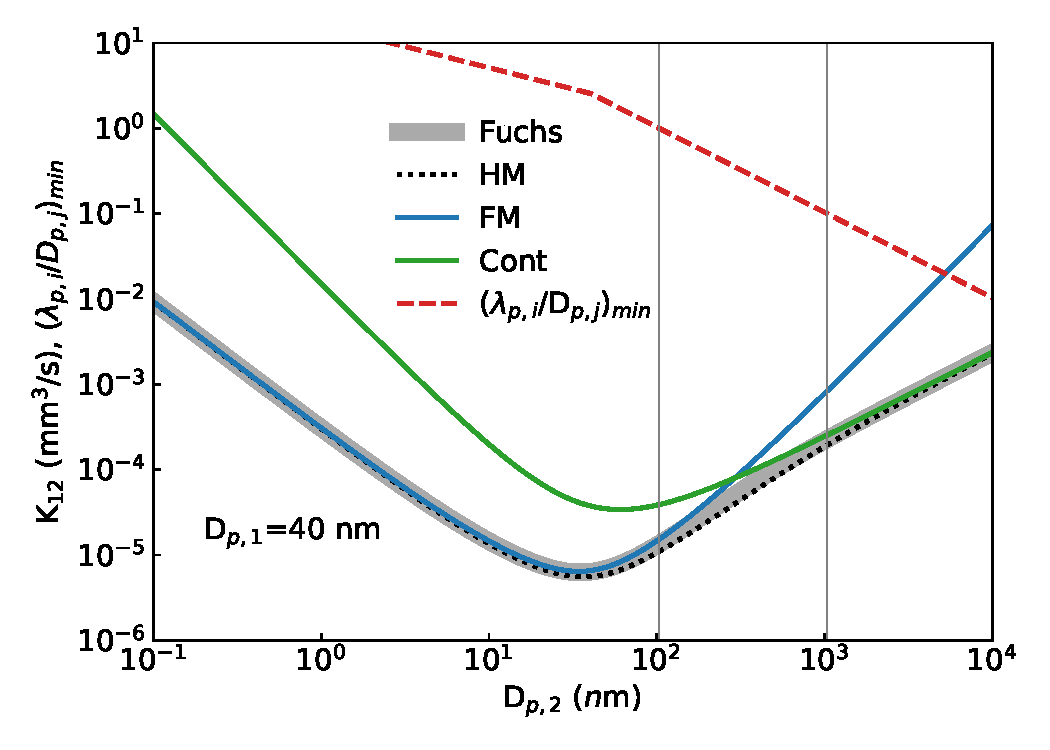
\includegraphics[width=0.8\textwidth]{fig_coagulation.pdf}
    \end{center}
    \caption{Coagulation coefficient $K_{12}$ for $D_{p,1}$=40 nm.}
    \label{f:coagulation}
\end{figure}
%

SootLib implements four soot coagulation mechanisms derived from the models above. Users can choose the continuum limit (\texttt{CONTINUUM}), the free-molecular limit (\texttt{FM}), the harmonic mean representation of the transition regime (\texttt{HM}), or the Fuchs form of the coagulation coefficient (\texttt{FUCHS}).

%%%%%%%%%%%%%%%%%%%%%%%%%%%%%%%%%%%%%%%%%%%%%%%%%%%%%%%%%%%%%%%%%%%%%%%%%%%%%%%

\subsection{Particle size distribution and dynamics}
\label{s:PSD_dynamics}

There are two common approaches to modeling aerosol particle size distributions (PSD): sectional and moment methods. Sectional methods divide the domain of particle sizes into discrete ranges based on, e.g., size or mass, while moment methods use the statistical moments of the soot PSD to describe the distribution. In both cases, transport equations defined by the soot variables (sections or moments) interact with the soot chemistry mechanisms to represent the soot evolution during a simulation. Table~\ref{t:psd_models} summarizes the PSD treatments implemented in SootLib.
%
\begin{table}
    \caption{Summary of soot particle size distribution models implemented in SootLib.}
    \label{t:psd_models}
    \centering
    \resizebox{\textwidth}{!}{
        \begin{tabular}{l l l}
            \toprule
            PSD model                                    & Model ID & \# Moments   \\
            \midrule
            Monodisperse~\cite{Lignell_2008b}     & \texttt{MONO}  & 2      \\
            Lognormal~\cite{Lignell_2008b}        & \texttt{LOGN}  & 3  \\
            Quadrature method of moments~\cite{McGraw_1997,Marchisio_2013} & \texttt{QMOM}  & 2, 4, 6, 8  \\
            Method of moments with interpolative closure~\cite{Frenklach_2002b} & \texttt{MOMIC} & 3\textendash8  \\
            Sectional model~\cite{Lehtinen_2001} & \texttt{SECT} & N/A \\
            \bottomrule
        \end{tabular}
    }
\end{table}
%

%%%%%%%%%%%%%%%%%%%%%%%%%%%%%%%%%%%%%%%%%%%%%%%%%%%%%%%%%%%%%%%%%%%%%%%%%%%%%%%

\subsubsection{Moment methods}
\label{s:moment-methods}

Moment methods describe the PSD using the statistical moments of the distribution. The $k^{th}$ using a discrete PSD is defined by
%
\begin{equation}
    M_k = \sum_i m_i^kN_i,
\end{equation}
%
where the summation is over all possible sizes, and $m_i$ and $N_i$ are the mass (kg) and number density (\#/m$^3$), of size $i$, respectively. For a continuous distribution $M_k$ is defined as
%
\begin{equation} \label{e:mk}
    M_k = \int_0^\infty mn(m)dm,
\end{equation}
%
where $n(m)$ is the number density per unit mass so that $n(m)dm$ is the number of particles per volume between sizes $m$ and $m+dm$.
In most practical applications, only a small number of moments (2--8) is required to describe the full PSD so that moment methods are computationally more efficient than sectional methods. 

While moments are defined in terms of the PSD, that PSD is unknown and moment source terms must be written directly in terms of the moments, resulting in a closure problem. The closure approach used gives rise to different versions of the method of moments (MOM). For example a transport equation (unsteady in physical space) for soot number density with transport operator $\Gamma$ may be written
as
%
\begin{equation}
    \Gamma(n(m)) = \dot{N} + \dot{G} + \dot{C},
\end{equation}
%
where $\dot{N}$, $\dot{G}$, and $\dot{C}$ are source terms for nucleation, net growth, and coagulation, respectively, which are functions of $n(m)$. The transport equation for $M_k$ is 
%
\begin{equation}
    \Gamma(M_k) = \underbrace{\int_0^\infty m^k\dot{N}dm}_{\dot{N}_k} + 
    \underbrace{\int_0^\infty m^k\dot{G}dm}_{\dot{G}_k}+ 
    \underbrace{\int_0^\infty m^k\dot{C}dm}_{\dot{C}_k}.
\end{equation}
%
Consider the net growth term; it is given by $\dot{G} = -\prtl{ }{m}(v_gn)$, where $v_g=k_s\pi(6/\pi\rho_s)^{2/3}m^{2/3}$ is the growth velocity in the mass coordinate, $k_s$ is the chemical growth rate per unit area, and $\rho_s$ is the soot density. Integrating by parts gives $\dot{G}_k=k\int_0^\infty v_gm^{k-1}n(m)dm$, and insertion of $v_g$ and using the moment definition gives
%
\begin{equation}
    \dot{G}_k = k_s\pi\left(\frac{6}{\pi \rho_s}\right)^{2/3}kM_{k-1/3}.
\end{equation}
%
Transporting integer $k$ moments requires closure of fractional moments $M_{k-1/3}$. Other source terms require similar closures (not shown).

The monodispersed model (\texttt{MONO}) assumes $n(m)=\delta(m-\bar{m})$, where $\bar{m}=M_1/M_0$ and only $M_0$ (the total number of all particles per volume) and $M_1$ (the mass density of soot particles) are considered. The \texttt{LOGN} model assumes the PSD is lognormal~\cite{Pratsinis_1988}. In this case, fractional moments are given in terms of the first three integer moments $M_0$, $M_1$, and $M_2$~\cite{Lignell_2008b}
%
\begin{equation}
    M_k = M_0^{1-\frac{3}{2}k+\frac{1}{2}k^2} M_1^{2k-k^2} M_2^{\frac{1}{2}k^2-\frac{1}{2}k}.
\end{equation}
%
The quadrature method of moments (\texttt{QMOM}) assumes the PSD is given by
%
\begin{equation} \label{e:nqmom}
    n(m) = \sum_{\alpha=1}^{N_e}w_\alpha\delta(m-m_\alpha),
\end{equation}
%
where $N_e$ is the number of particle \emph{environments}, (half the number of moments considered), and $w_\alpha$ and $m_\alpha$ are the number density and particle mass in environment $\alpha$, which can be solved algebraically~\cite{Wheeler_1974, Marchisio_2013} using Eqs.~(\ref{e:mk},\ref{e:nqmom}). Given the assumed forms for $n(m)$ in these three PSD models, the integrals in the moment source terms can be directly evaluated.

The method of moments with interpolative closure (MOMIC) avoids specifying the shape of the soot PSD and closes the moment source terms by interpolating between whole order moments to calculate fractional moments. 
SootLib implements MOMIC as described by Frenklach~\cite{Frenklach_2002b,Frenklach_1987}
using polynomial interpolation between logarithms of the whole-order moments. The form of the free molecular coagulation coefficient requires special treatment in both MOMIC and the lognormal closure approaches as described in the source documentation and literature.

%%%%%%%%%%%%%%%%%%%%%%%%%%%%%%%%%%%%%%%%%%%%%%%%%%%%%%%%%%%%%%%%%%%%%%%%%%%%%%%

\subsubsection{Sectional model}
\label{s:sectional}

Sectional models represent the PSD directly---rather than through its statistical moments---using the particle number density in a defined set of sections (or \emph{bins}) that represent the discretized domain. In the \texttt{SECT} model, the desired number of bins are spaced geometrically by a variable by default factor of two.

Sectional models do not require the same type of closure that moment methods do, but coagulation between particles usually results in particles with sizes between given section sizes. Since the particles can only reside in the given sections, the intermediate size is modeled by assigning a number of particles to each of the two neighboring sections so that total mass and number are conserved~\cite{Lehtinen_2001}. Any particles formed that are larger than the last section are placed in that section in an amount to conserve mass. Growth and oxidation are represented by a velocity in the size coordinate. SootLib uses an upwind method to maintain stability, but higher order monotone schemes for conservation laws (e.g., flux limiters) can implemented.

The advantage of the sectional model over the MOM is that it gives a direct representation of the PSD, and is potentially more accurate if sufficient resolution is included. The disadvantage is the many more sections (and hence soot variables) are required than is typical in the MOM. In both cases, $M_0$ and $M_1$ are the primary variables of interest, with $M_1/\rho_s$ being the soot volume fraction that is most commonly measured experimentally.

%%%%%%%%%%%%%%%%%%%%%%%%%%%%%%%%%%%%%%%%%%%%%%%%%%%%%%%%%%%%%%%%%%%%%%%%%%%%%%%

\subsection{Model combinations and limitations}
\label{s:limitations}

SootLib is designed to be semi-modular in that the various soot chemistry mechanisms can be substituted and exchanged, providing users with increased flexibility. It must be noted, however, that not all model combinations will produce physically meaningful results, either due to a model's design or its author's intent. The following notes indicate some limitations to be aware of when choosing model combinations.

SootLib computes soot variable source terms using a specified gas and soot variable state, usually as part of separate reacting flow simulation tool, such as for a premixed flame, in which energy and gas composition profiles are solved. In this case, the gas-phase chemistry mechanism should include the species required by the chosen soot chemistry mechanisms. However, SootLib is fully independent of such a gas mechanism, and the gas composition vector SootLib uses is whatever the user provides.  

The following points apply to model specification:
\begin{itemize}
\item The \texttt{LL} model is included with SootLib as a point of reference because it is common in combustion simulation studies. This model was developed from experimental ethylene jet flames, and its accuracy and applicability are generally limited to conditions similar to those under which it was developed.
\item The \texttt{HACA} surface growth and oxidation mechanisms should not be used separately. The code will give a warning otherwise.
\item The \texttt{PAH} nucleation mechanism also results in PAH condensation~\cite{Blanquart_2009c}; these may be separated in a future release.
\item The \texttt{PAH} nucleation mechanism assumes that the self-collision of PAH molecules occurs in the free-molecular regime independent of the coagulation model specified by the user.
\end{itemize}
%

Regarding the PSD model chosen, \texttt{QMOM} requires an even number of moments. The \texttt{MONO} and \texttt{QMOM} with two moments are verified to give identical results, but the \texttt{MONO} is simpler and has somewhat less computational overhead. Both \texttt{MOMIC} and \texttt{QMOM} are limited to eight moments, but no more than six should generally be needed.

%%%%%%%%%%%%%%%%%%%%%%%%%%%%%%%%%%%%%%%%%%%%%%%%%%%%%%%%%%%%%%%%%%%%%%%%%%%%%%%

\section{Software description}
\label{s:architecture}

SootLib is an object-oriented C++ library intended for use in reacting flow simulations including CFD.
Upon download, the SootLib package contains four directories: 
%
\begin{itemize}
    \item \texttt{src} contains the SootLib source code; 
    \item \texttt{examples} contains usage example codes; 
    \item \texttt{tests} contains SootLib's optional testing suite, driven by Catch2; and 
    \item \texttt{docs} contains the files optionally used to generate code documentation with Doxygen.
\end{itemize}
%
SootLib installation is automated by CMake, and project options can be changed by editing the top-level \texttt{CMakeLists.txt} file or by editing the \texttt{CMakeCache.txt} file. Refer to the package documentation for detailed compilation and installation instructions, including a full list of CMake options.

Successful installation will generate an \texttt{include/sootlib} directory that contains SootLib's header files and a \texttt{lib} directory that contains the library file, \texttt{libsootModel.a} and SootLib's relocatable CMake package, \texttt{sootlib.cmake}.
To use SootLib in C++ code, include the installed header file \texttt{sootHeaders.h} and link the \texttt{libsootModel.a} library file. Alternately, SootLib can also be used as part of larger CMake projects via \texttt{sootlib.cmake} or CMake's FetchContent module.

The SootLib library consists primarily of two object classes through which the user interacts with the library---\texttt{state} and \texttt{sootModel}---both of which are contained within the \texttt{soot} namespace. The \texttt{state} object holds user-supplied details about the current thermodynamic state: temperature, pressure, density, viscosity, gas species mass fractions, and soot variable quantities (a vector of moments or section number densities). The \texttt{sootModel} object contains information about the selected models and performs the calculations that generate source terms for the sectional or moment transport equations. The \texttt{sootModel} is constructed by setting the number of soot variables and the desired nucleation, growth, oxidation, and coagulation models. Those models can be set either through an enumeration variable or by creating the respective model objects.
The resulting soot and gas species source terms are accessed via the \texttt{sootModel} object's \texttt{sourceTerms} struct called \texttt{sources}. Refer to the package documentation and examples for further details on using the SootLib library.

SootLib's two major functionalities are:
\begin{itemize}
    \item Calculates source terms for the soot transport equations given thermodynamic state details and chemistry mechanisms chosen by the user; and
    \item Calculates mass source terms for gaseous chemical species affected by soot chemistry.
\end{itemize}

%%%%%%%%%%%%%%%%%%%%%%%%%%%%%%%%%%%%%%%%%%%%%%%%%%%%%%%%%%%%%%%%%%%%%%%%%%%%%%%

\section{Examples}
\label{s:examples}

Two examples are provided with SootLib. 
\texttt{simple\textunderscore example.cc} is provided as a basic, standalone example of soot model setup, source term calculation, and source term retrieval to illustrate use of the SootLib library. This format has limited functionality, but can be useful for directly comparing various models' source term calculations. 
It is primarily intended as an illustration of how to set up and interact with the library. The second example is a burner-stabilized premixed flame.

\subsection{Premixed burner example}
\label{s:soot-examples-premixed}

By way of demonstration, we coupled SootLib with the one-dimensional burner stabilized premixed flame code in Cantera~\cite{Cantera}. We consider ISF laminar premixed flame 2~\cite{ISF4-P2}, an ethylene--air fuel mixture with an equivalence ratio $\phi=2.34$ flowing at a velocity of \qty{6.73}{\cm/\s}---and compare simulation results to the three sets of experimental data provided in this configuration~\cite{Xu_1997,Menon_2007}.

The simulation case used the GRI 3.0 gas chemistry mechanism~\cite{Smith_2002}. Soot chemistry is described with the \texttt{LIN} nucleation mechanism~\cite{Lindstedt_2005}, \texttt{LIN} surface growth~\cite{Lindstedt_1994}, \texttt{LL} oxidation~\cite{Leung_1991}, free-molecular coagulation~\cite{Seinfeld_2016}, and the monodisperse PSD model (\texttt{MONO}).

Figure~\ref{f:soot-premix} shows the simulation results for soot volume fraction as a function of height above the burner surface along with experimental values. 
The simulation results agree well with the experimental data though there is significant variation in the experimental soot volume fraction. The soot model used kinetic data fitted to experiments of diffusion flames and assumed free molecular coagulation. The soot volume fraction is about an order of magnitude higher at high burner heights if the harmonic mean or Fuchs coagulation models are used instead, which results in more particles and more surface area for growth.
%
\begin{figure}
    \begin{center}
        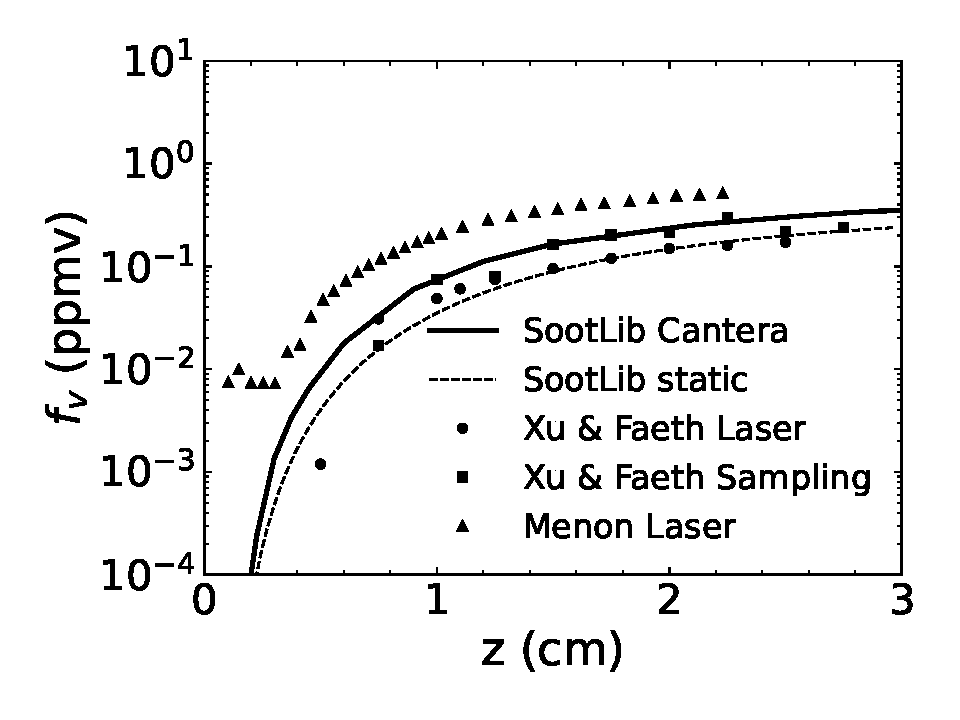
\includegraphics[width=0.8\textwidth]{fig_burner.pdf}
    \end{center}
    \caption{Premixed burner flame comparing simulation to experimental data.}
    \label{f:soot-premix}
\end{figure}
%

SootLib provides a second example \texttt{burner\textunderscore flame.cc} that integrates soot variables using static temperature, velocity, density, viscosity, and gas mass fraction profiles from the Cantera simulation discussed above. This gives a relevant example while allowing independence from third-party simulation codes. The soot equations solved are $dM_k/dz = \dot{M}_k/\rho v$, where $\rho$ and $v$ are the gas density and velocity profiles. Differences between the two simulations are due to neglecting diffusion effects and gas-soot coupling in the static simulation.

Figure~\ref{f:sectional} shows the \texttt{burner\textunderscore flame.cc} example output using the sectional model with 40 soot sizes. The size distribution is shown at eight burner heights showing its evolution from the power-law nucleation mode at early times to including the lognormally-distributed coagulation mode at later times.
%
\begin{figure}
    \begin{center}
        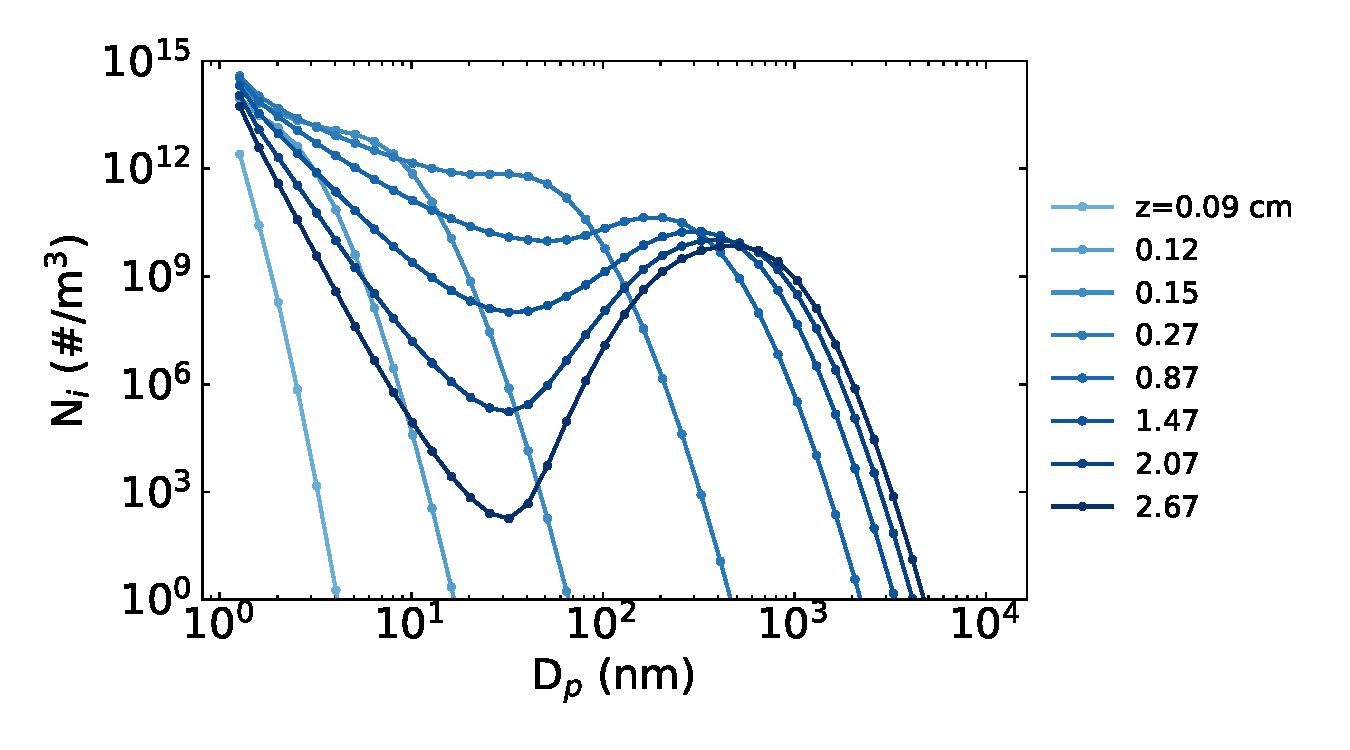
\includegraphics[width=0.8\textwidth]{fig_sectional.pdf}
    \end{center}
    \caption{Premixed burner flame using the sectional model showing the evolution of the PSD.}
    \label{f:sectional}
\end{figure}
%

Computational cost comparisons of the various models have been performed. These results are presented in the source documentation files (Doxygen).

%%%%%%%%%%%%%%%%%%%%%%%%%%%%%%%%%%%%%%%%%%%%%%%%%%%%%%%%%%%%%%%%%%%%%%%%%%%%%%%

\section{Conclusion}
\label{s:soot-conclusion}

To the authors' best knowledge, there is no existing tool like SootLib, which combines various soot models into one package on a consistent, cross-platform, open-source framework that is not specific to any one CFD code or simulation type. It requires no external dependencies except for LApack, and it can be used in C++ projects directly or included in larger CMake projects via its exported package or CMake's FetchContent module. Users interact with the SootLib library through a small group of objects and functions that allow them to specify model parameters, set a thermodynamic state and composition for the gas environment, and calculate source terms for moment transport equations.

SootLib is intended to be a convenient tool that provides combustion researchers with more options and more control over simulations involving sooting flames. For researchers who do not specialize in soot but require soot modeling in order to perform accurate simulations, SootLib lowers the barrier to entry on the topic; it requires a minimum of prior knowledge to use, representing a significant time savings to its users. For combustion researchers who do specialize in soot, SootLib's uniform framework and modular design make it a good comparative tool, increasing the potential for useful parametric studies involving soot and decreasing the overhead involved with testing new and existing soot models under a variety of conditions.

SootLib has been implemented into both Cantera~\cite{Cantera} and in the One-Dimensional Turbulence ODT code~\cite{Stephens_2021}. 

%%%%%%%%%%%%%%%%%%%%%%%%%%%%%%%%%%%%%%%%%%%%%%%%%%%%%%%%%%%%%%%%%%%%%%%%%%%%%%%

\section{Conflict of Interest}

The authors declare that they have no known competing financial interests or personal relationships that could have appeared to influence the work reported in this paper.

%%%%%%%%%%%%%%%%%%%%%%%%%%%%%%%%%%%%%%%%%%%%%%%%%%%%%%%%%%%%%%%%%%%%%%%%%%%%%%%

\section*{Acknowledgements}

This research was supported in part by the National Science Foundation under grant number CBET-1403403.

%%%%%%%%%%%%%%%%%%%%%%%%%%%%%%%%%%%%%%%%%%%%%%%%%%%%%%%%%%%%%%%%%%%%%%%%%%%%%%%

%% References:

\begin{thebibliography}{10}
\expandafter\ifx\csname url\endcsname\relax
  \def\url#1{\texttt{#1}}\fi
\expandafter\ifx\csname urlprefix\endcsname\relax\def\urlprefix{URL }\fi
\expandafter\ifx\csname href\endcsname\relax
  \def\href#1#2{#2} \def\path#1{#1}\fi

\bibitem{EPA_2009}
{National Center for Environmental Assessment Office of Research and
  Development}, {Integrated Science Assessment for Particulate Matter} (2009).

\bibitem{EPA_2004}
{National Center for Environmental Assessment Office of Research and
  Development}, {Air Quality Criteria for Particulate Matter} (2004).

\bibitem{Pope_2000}
S.~B. Pope, {Turbulent Flows}, {Cambridge University Press}, 2000.

\bibitem{Frenklach_2002b}
M.~Frenklach, {Method of moments with interpolative closure}, {Chemical
  Engineering Science} 57~(12) (2002) 2229--2239.
\newblock \href {http://dx.doi.org/10.1016/S0009-2509(02)00113-6}
  {\path{doi:10.1016/S0009-2509(02)00113-6}}.

\bibitem{Jullien_1987}
R.~Jullien, R.~Botet, {Aggregation and Fractal Aggregates}, {World Scientific
  Publishing}, 1987.

\bibitem{Wang_2011}
H.~Wang, {Formation of nascent soot and other condensed-phase materials in
  flames}, {Proceedings of the Combustion Institute} 33~(1) (2011) 41--67.
\newblock \href {http://dx.doi.org/10.1016/j.proci.2010.09.009}
  {\path{doi:10.1016/j.proci.2010.09.009}}.

\bibitem{Leung_1991}
K.~M. Leung, R.~P. Lindstedt, W.~P. Jones, {A simplified reaction mechanism for
  soot formation in nonpremixed flames}, {Combustion and Flame} 87 (1991)
  289--305.
\newblock \href {http://dx.doi.org/10.1016/0010-2180(91)90114-q}
  {\path{doi:10.1016/0010-2180(91)90114-q}}.

\bibitem{Lindstedt_2005}
R.~P. Lindstedt, H.~Ozarovsky, {Joint scalar transported {PDF} modeling of
  nonpiloted turbulent diffusion flames}, {Combustion and Flame} 143~(4) (2005)
  471--490.
\newblock \href {http://dx.doi.org/10.1016/j.combustflame.2005.08.030}
  {\path{doi:10.1016/j.combustflame.2005.08.030}}.

\bibitem{Blanquart_2009}
G.~Blanquart, P.~Pepiot-Desjardins, H.~Pitsch, {Chemical mechanism for high
  temperature combustion of engine relevant fuels with emphasis on soot
  precursors}, {Combustion and Flame} 156~(3) (2009) 588--607.
\newblock \href {http://dx.doi.org/10.1016/j.combustflame.2008.12.007}
  {\path{doi:10.1016/j.combustflame.2008.12.007}}.

\bibitem{Lindstedt_1994}
R.~P. Lindstedt, {Simplified soot nucleation and surface growth steps for
  non-premixed flames}, in: H.~Bockhorn (Ed.), {Soot Formation in Combustion},
  no.~59 in {Springer Series in Chemical Physics}, {Springer-Verlag Berlin
  Heidelberg}, 1994, pp. 417--441.

\bibitem{Appel_2000}
J.~Appel, H.~Bockhorn, M.~Frenklach, {Kinetic modeling of soot formation with
  detailed chemistry and physics: laminar premixed flames of C2 hydrocarbons},
  {Combustion and Flame} 121~(1-2) (2000) 122--136.
\newblock \href {http://dx.doi.org/10.1016/S0010-2180(99)00135-2}
  {\path{doi:10.1016/S0010-2180(99)00135-2}}.

\bibitem{Frenklach_1994}
M.~Frenklach, H.~Wang, {Detailed mechanism and modeling of soot particle
  formation}, in: H.~Bockhorn (Ed.), {Soot Formation in Combustion}, no.~59 in
  {Springer Series in Chemical Physics}, {Springer-Verlag Berlin Heidelberg},
  1994, pp. 165--192.

\bibitem{Lee_1962}
B.~J. Lee, M.~W. Thring, J.~M. Be{\'e}r, {On the rate of combustion of soot in
  a laminar soot flame}, {Combustion and Flame} 6 (1962) 137--145.
\newblock \href {http://dx.doi.org/10.1016/0010-2180(62)90082-2}
  {\path{doi:10.1016/0010-2180(62)90082-2}}.

\bibitem{Neoh_1980}
K.~G. Neoh, {Soot Burnout in Flames}, {PhD}, {Massachusetts Institute of
  Technology} (1980).

\bibitem{Neoh_1981}
K.~G. Neoh, J.~B. Howard, A.~F. Sarofim, {Soot Oxidation in Flames}, in: D.~C.
  Siegla, G.~W. Smith (Eds.), {Particulate Carbon: Formation During
  Combustion}, {Springer US}, 1981, pp. 261--282.
\newblock \href {http://dx.doi.org/10.1007/978-1-4757-6137-5_9}
  {\path{doi:10.1007/978-1-4757-6137-5_9}}.

\bibitem{Nagle_1962}
J.~Nagle, R.~F. Strickland-Constable, {Oxidation of carbon between
  1000--2000C}, in: S.~Mrozowski, M.~L. Studebaker, P.~L. Walker (Eds.),
  {Proceedings of the Fifth Conference on Carbon}, no.~1, {Pennsylvania State
  University}, {Pergamon Press}, 1962, pp. 154--164.

\bibitem{Seinfeld_2016}
J.~H. Seinfeld, S.~N. Pandis, {Atmospheric Chemistry and Physics}, third
  edition Edition, {John Wiley {\&} Sons}, 2016.

\bibitem{Fuchs_1964}
N.~Fuchs, {The Mechanics of Aerosols}, revised and enlarged edition Edition,
  Vol.~91, {Pergamon Press}, 1964.
\newblock \href {http://dx.doi.org/10.1002/qj.49709138822}
  {\path{doi:10.1002/qj.49709138822}}.

\bibitem{Blanquart_2009c}
G.~Blanquart, H.~Pitsch, {A joint volume-surface-hydrogen multi-variate model
  for soot formation}, in: H.~Bockhorn, A.~D'Anna, A.~F. Sarofim, H.~Wang
  (Eds.), {Combustion Generated Fine Carbonaceous Particles}, {KIT Scientific
  Publishing}, 2009, pp. 437--463.

\bibitem{Harris_1988}
S.~J. Harris, I.~M. Kennedy, The coagulation of soot particles with van der
  waals forces, Combustion Science and Technology 59~(4-6) (1988) 443--454.
\newblock \href {http://dx.doi.org/10.1080/00102208808947110}
  {\path{doi:10.1080/00102208808947110}}.

\bibitem{Kazakov_1998}
A.~Kazakov, M.~Frenklach, {Dynamic Modeling of Soot Particle Coagulation and
  Aggregation: Implementation With the Method of Moments and Application to
  High-Pressure Laminar Premixed Flames}, {Combustion and Flame} 114~(3-4)
  (1998) 484--501.
\newblock \href {http://dx.doi.org/10.1016/S0010-2180(97)00322-2}
  {\path{doi:10.1016/S0010-2180(97)00322-2}}.

\bibitem{Lignell_2008b}
D.~O. Lignell, {Direct Numerical Simulation of Soot Formation and Transport In
  Turbulent Nonpremixed Ethylene Flames}, {PhD}, {The University of Utah}
  (2008).

\bibitem{McGraw_1997}
R.~McGraw, {Description of Aerosol Dynamics by the Quadrature Method of
  Moments}, {Aerosol Science and Technology} 27~(2) (1997) 255--265.
\newblock \href {http://dx.doi.org/10.1080/02786829708965471}
  {\path{doi:10.1080/02786829708965471}}.

\bibitem{Marchisio_2013}
D.~L. Marchisio, R.~O. Fox, {Computational Models for Polydisperse Particulate
  and Multiphase Systems}, {Cambridge University Press}, 2013.
\newblock \href {http://dx.doi.org/10.1017/CBO9781139016599}
  {\path{doi:10.1017/CBO9781139016599}}.

\bibitem{Lehtinen_2001}
K.~E.~J. Lehtinen, M.~R. Zachariah, {Self-Preserving Theory for the Volume
  Distribution of Particles Undergoing Brownian Coagulation}, {Journal of
  Colloid and Interface Science} 242~(2) (2001) 314--318.
\newblock \href {http://dx.doi.org/10.1006/jcis.2001.7791}
  {\path{doi:10.1006/jcis.2001.7791}}.

\bibitem{Pratsinis_1988}
S.~E. Pratsinis, Simultaneous nucleation, condensation, and coagulation in
  aerosol reactors, Journal of Colloid and Interface Science 124~(2) (1988)
  416--427.

\bibitem{Wheeler_1974}
J.~C. Wheeler, {Modified moments and Gaussian quadratures}, {Rocky Mountain
  Journal of Mathematics} 4~(2).
\newblock \href {http://dx.doi.org/10.1216/RMJ-1974-4-2-287}
  {\path{doi:10.1216/RMJ-1974-4-2-287}}.

\bibitem{Frenklach_1987}
M.~Frenklach, S.~J. Harris, {Aerosol dynamics modeling using the method of
  moments}, {Journal of Colloid and Interface Science} 118~(1) (1987) 252--261.
\newblock \href {http://dx.doi.org/10.1016/0021-9797(87)90454-1}
  {\path{doi:10.1016/0021-9797(87)90454-1}}.

\bibitem{Cantera}
D.~G. Goodwin, H.~K. Moffat, I.~Schoegl, R.~L. Speth, B.~W. Weber, Cantera: An
  object-oriented software toolkit for chemical kinetics, thermodynamics, and
  transport processes, \url{https://www.cantera.org}, version 2.6.0 (2022).
\newblock \href {http://dx.doi.org/10.5281/zenodo.6387882}
  {\path{doi:10.5281/zenodo.6387882}}.

\bibitem{ISF4-P2}
G.~Nathan,
  \href{https://www.adelaide.edu.au/cet/isfworkshop/data-sets/laminar-flames}{{International
  Sooting Flame Workshop}} (2023).
\newline\urlprefix\url{https://www.adelaide.edu.au/cet/isfworkshop/data-sets/laminar-flames}

\bibitem{Xu_1997}
F.~Xu, {Soot formation in laminar premixed ethylene/air flames at atmospheric
  pressure}, {Combustion and Flame} 108~(4) (1997) 471--493.
\newblock \href {http://dx.doi.org/10.1016/S0010-2180(96)00200-3}
  {\path{doi:10.1016/S0010-2180(96)00200-3}}.

\bibitem{Menon_2007}
A.~V. Menon, S.-Y. Lee, M.~J. Linevsky, T.~A. Litzinger, R.~J. Santoro,
  {Addition of NO2 to a laminar premixed ethylene--air flame: Effect on soot
  formation}, {Proceedings of the Combustion Institute} 31~(1) (2007) 593--601.
\newblock \href {http://dx.doi.org/10.1016/j.proci.2006.08.105}
  {\path{doi:10.1016/j.proci.2006.08.105}}.

\bibitem{Smith_2002}
G.~P. Smith, M.~Frenklach, N.~W. Moriarty, B.~Eiteneer, M.~Goldenberg, C.~T.
  Bowman, R.~K. Hanson, S.~Song, W.~C. Gardiner, V.~V. Lissianski, Z.~Qin,
  D.~M. Golden, \href{http://combustion.berkeley.edu/gri-mech/}{{GRI-Mech 3.0}}
  (2002).
\newline\urlprefix\url{http://combustion.berkeley.edu/gri-mech/}

\bibitem{Stephens_2021}
V.~B. Stephens, D.~O. Lignell, {One-dimensional turbulence ({ODT}):
  computationally efficient modeling and simulation of turbulent flows},
  {SoftwareX} 13.
\newblock \href {http://dx.doi.org/10.1016/j.softx.2020.100641}
  {\path{doi:10.1016/j.softx.2020.100641}}.

\end{thebibliography}

%%%%%%%%%%%%%%%%%%%%%%%%%%%%%%%%%%%%%%%%%%%%%%%%%%%%%%%%%%%%%%%%%%%%%%%%%%%%%%%

\section*{Required Metadata}

\section*{Current code version}

Ancillary data table required for subversion of the codebase. Kindly replace examples in right column with the correct information about your current code, and leave the left column as it is.

\begin{table}
\begin{tabular}{|l|p{6.5cm}|p{6.5cm}|}
\hline
\textbf{Nr.} & \textbf{Code metadata description} & \textbf{Please fill in this column} \\
\hline
C1 & Current code version & 1.0 \\
\hline
C2 & Permanent link to code/repository used for this code version & https://github.com/byuignite/sootlib \\
\hline
C3  & Permanent link to Reproducible Capsule & \\
\hline
C4 & Legal Code License & MIT \\
\hline
C5 & Code versioning system used & Git \\
\hline
C6 & Software code languages, tools, and services used & C++ \\
\hline
C7 & Compilation requirements, operating environments \& dependencies & C++11, CMake 3.15+\\
\hline
C8 & If available Link to developer documentation/manual &  \\
\hline
C9 & Support email for questions & davidlignell@byu.edu \\
\hline
\end{tabular}
\caption{Code metadata (mandatory)}
\end{table}

%\section*{Current executable software version}
%
%Ancillary data table required for sub version of the executable software: (x.1, x.2 etc.) kindly replace examples in right column with the correct information about your executables, and leave the left column as it is.
%
%\begin{table}
%\begin{tabular}{|l|p{6.5cm}|p{6.5cm}|}
%\hline
%\textbf{Nr.} & \textbf{(Executable) software metadata description} & \textbf{Please fill in this column} \\
%\hline
%S1 & Current software version & 1.0 \\
%\hline
%S2 & Permanent link to executables of this version  &  \\
%\hline
%S3  & Permanent link to Reproducible Capsule & \\
%\hline
%S4 & Legal Software License & MIT \\
%\hline
%S5 & Computing platforms/Operating Systems & Windows, MacOS, Linux \\
%\hline
%S6 & Installation requirements \& dependencies & C++11, CMake 3.15+, Catch2 (optional)\\
%\hline
%S7 & If available, link to user manual - if formally published include a reference to the publication in the reference list & \\
%\hline
%S8 & Support email for questions & davidlignell@byu.edu \\
%\hline
%\end{tabular}
%\caption{Software metadata (optional)}
%\end{table}

%%%%%%%%%%%%%%%%%%%%%%%%%%%%%%%%%%%%%%%%%%%%%%%%%%%%%%%%%%%%%%%%%%%%%%%%%%%%%%%

\end{document}
\endinput
